\section{Data Transfer}

\section*{Data Transfer Instructions}
\section*{Loading Data}
\begin{itemize}
  \item MOVS
  \item Reg to Reg MOVS R1, R2
  \item 8-Bit Literal MOVS R1,\#0x1C
  \item Constant MOVS R1, \#MyConst
  \item LDR
  \item 32-Bit Literal LDR R1, \#OxA1B2C3D4
  \item Literal + Offset LDR R1, [PC, \#12]
  \item Constant LDR R1, =MyConst
  \item Reg Value LDR R1, [R2]
  \item LDRB
  \item Load Register Byte
  \item Bits 31 to 8 set to zero
  \item LDRH
  \item Load Register Half-word
  \item Bits 31 to 16 set to zero
\end{itemize}

\section*{Load Array}
\begin{itemize}
  \item my\_array $=3$ * 4 Bytes
  \item Instructions $=5$ * 2 Bytes
  \item Literals (0x08) $=1 * 4$ Bytes\\
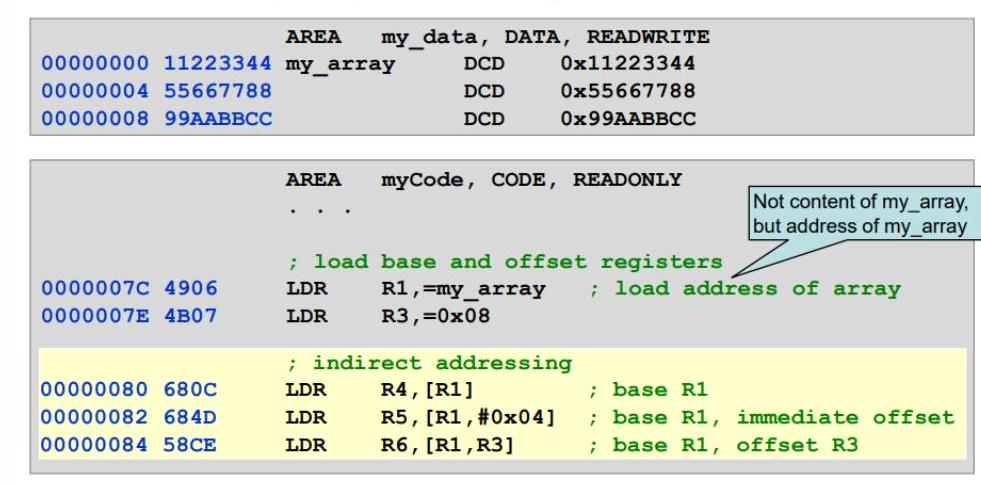
\includegraphics[width=\linewidth]{images/2024_12_29_79e6b22f503fb7b4f718g-03(1)}\\
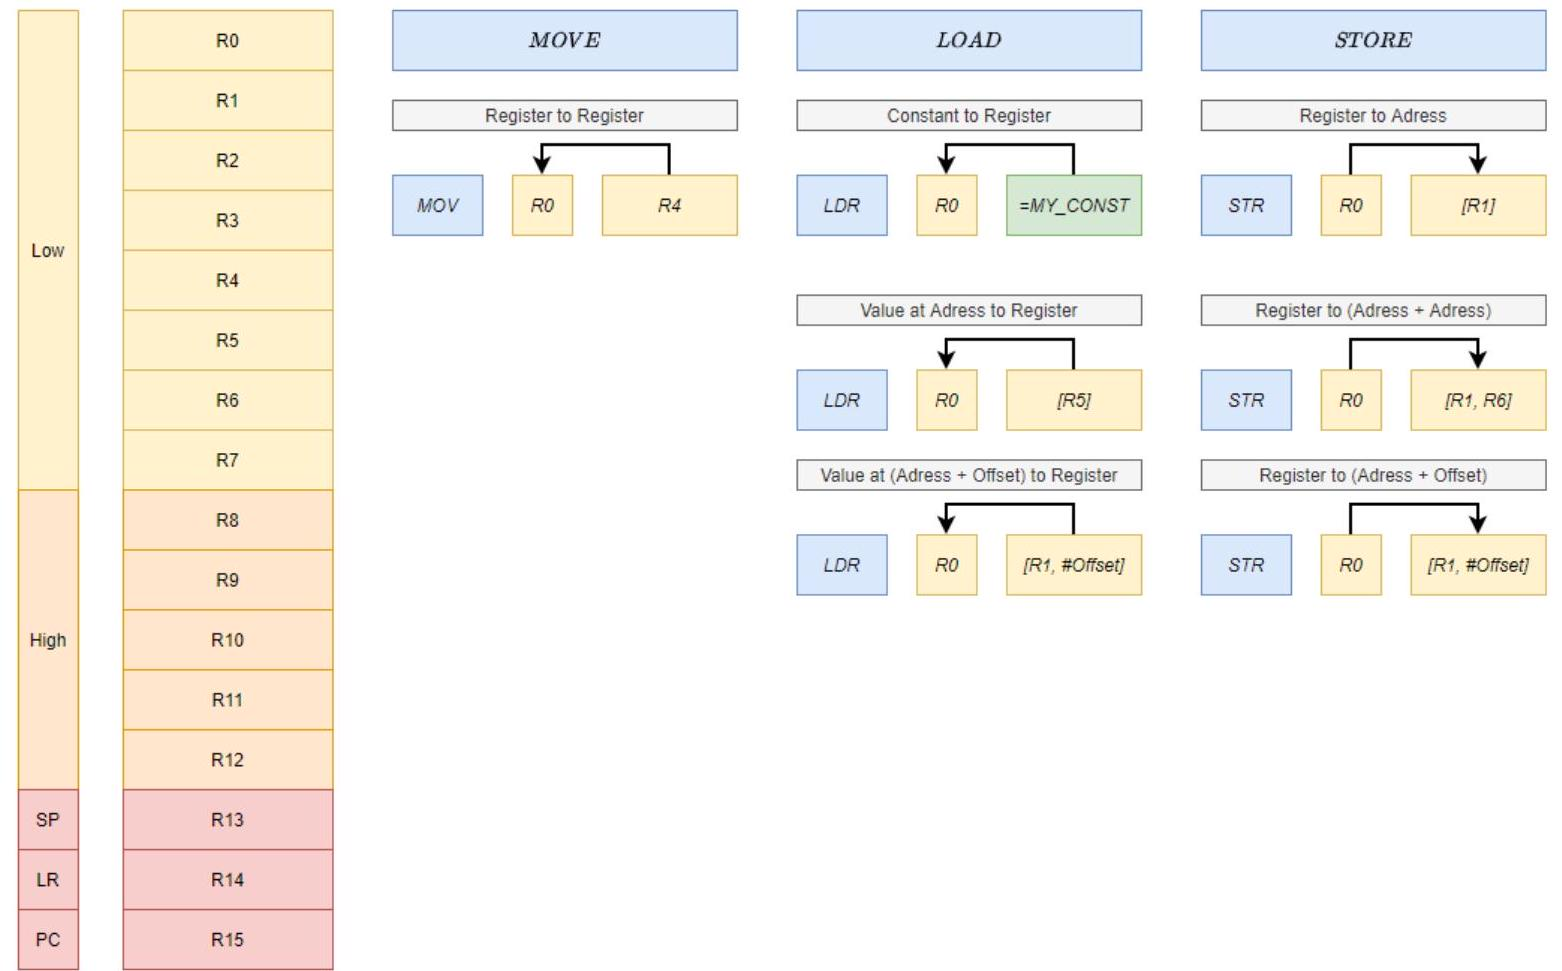
\includegraphics[width=\linewidth]{images/2024_12_29_79e6b22f503fb7b4f718g-03}
\end{itemize}

Storing Data

\begin{itemize}
  \item STR
  \item Value from Register STR R1, [R2]
  \item Value from Reg + Offset $S T R R 1,[R 2, \# 0 x 04]$
  \item STRB
  \item Store Register Byte (Low 8 bits of register stored)
  \item STRH
  \item Store Register Half-word (Low 15 bits of register stored)
\end{itemize}